\documentclass[11pt]{report}
\usepackage{graphicx}
\renewcommand{\bibname}{References}

\begin{document}

\section*{Meeting report (06/21/2019)}
Some remarks from meeting with Dr Ahmed Eldawy are:
\begin{itemize}
 \item The input for the DCEL construction cannot be just a set of nodes and edges as a representation of a planar graph.  The information of the faces has to be available in some way.
 \item The formal input for the DCEL construction should be a set of polygons. The segments of each polygons should be traversed in order to capture the face they belongs.
 \item An overlay operation will operate over a merged DCEL obtained from the DCEL representations of two sets of polygons.
 \item Figure~\ref{fig:overlay} illustrates the steps to get a merged DCEL prior to an overlay operation.
 \item The spatial predicates union, intersection and/or difference will be solved by traversing the merged DCEL and applying boolean operators over the labels of each face.
 \item The real advantage of a parallel DCEL construction will be the chance of run multiples spatial predicates over the same DCEL in linear time.
 \item The partition and merge strategy presented last week is viable as a Map-Reduce operation.  Actually, it follows a similar concept applied to construct Voronoi diagrams discussed in \cite{li_scalable_2019} (Dr Eldawy is co-author of this study).
 \item According with the literature, the intersection detection and segment generation should not be a cost operation by running the sweep line algorithm as a local step and using the appropriate partitoning.
\end{itemize}

\begin{figure}
    \centering
    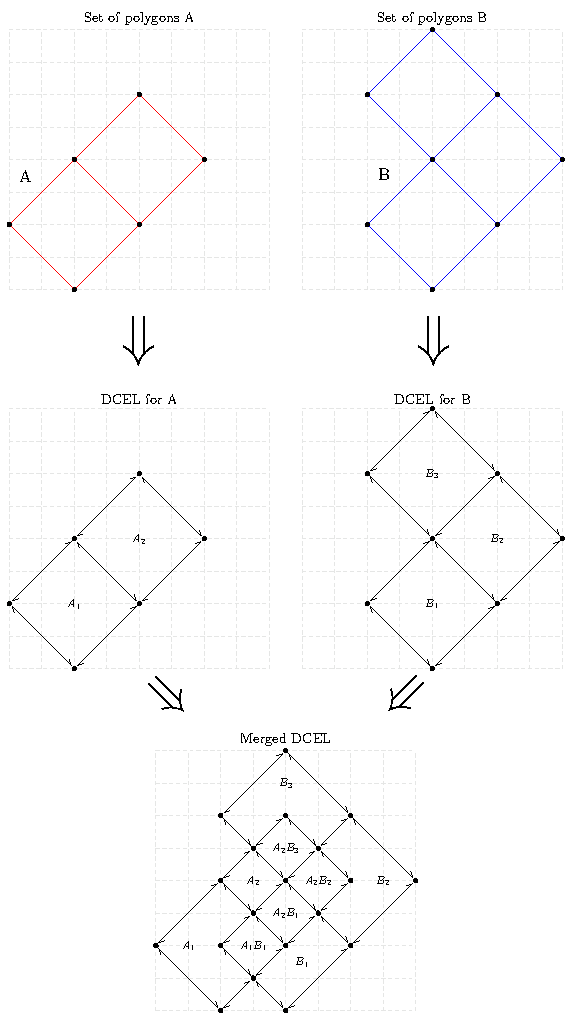
\includegraphics[width=0.79\textwidth]{Overlay}
    \caption{Merged DCEL prior to an overlay operation.}\label{fig:overlay}
\end{figure}

\bibliographystyle{unsrt}
\bibliography{dcel}
\end{document}
